\documentclass[]{article}
\usepackage{ listings} 
\usepackage{algorithm}
\usepackage{algorithmic}
\usepackage{graphicx}
\graphicspath{ {images/} }
\usepackage{float}
\usepackage{geometry}
\usepackage{pdfpages}

%opening
\title{}
\author{}
\date{}
\special{papersize=8.5in,11in}
\geometry{left=2cm,right=2cm,top=1.5cm,bottom=1.5cm}

\begin{document}

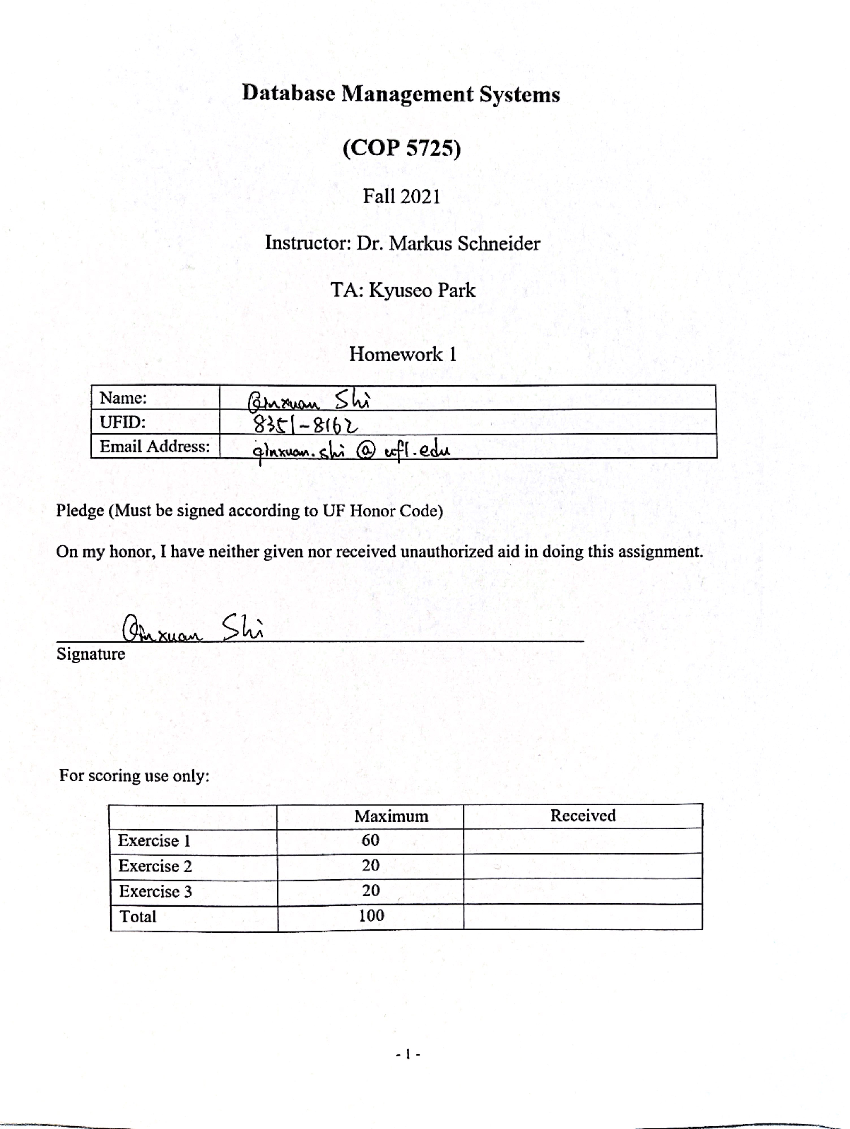
\includepdf{./document-H1/Homework.pdf}
\section{Exercise 1}

(1) SQL queries:
	\begin{lstlisting}[language=] 
	create TABLE ANIMAL_SHELTER(
	  AID VARCHAR(4),
	  ANIMAL_TYPE VARCHAR(10),
	  INTAKE_YEAR NUMBER(4),
	  INTAKE_CONDITION VARCHAR(10) check(
	 	INTAKE_CONDITION in ('Injured','Normal','Sick')
	  ),
	  NAME VARCHAR(10),
	  FOUND_LOCATION VARCHAR(25),
	  WEIGHT_UPON_INTAKE NUMERIC(4,1),
	  SEX_UPON_INTAKE VARCHAR(25) check(
	 	SEX_UPON_INTAKE in (
	 	  'Neutered Male','Intact Male','Spayed Female'
	 	)
	  ),
	  primary key (AID)
	);
	\end{lstlisting} 
	Output screen snapshots:
	\begin{figure}[H]
		\centering
		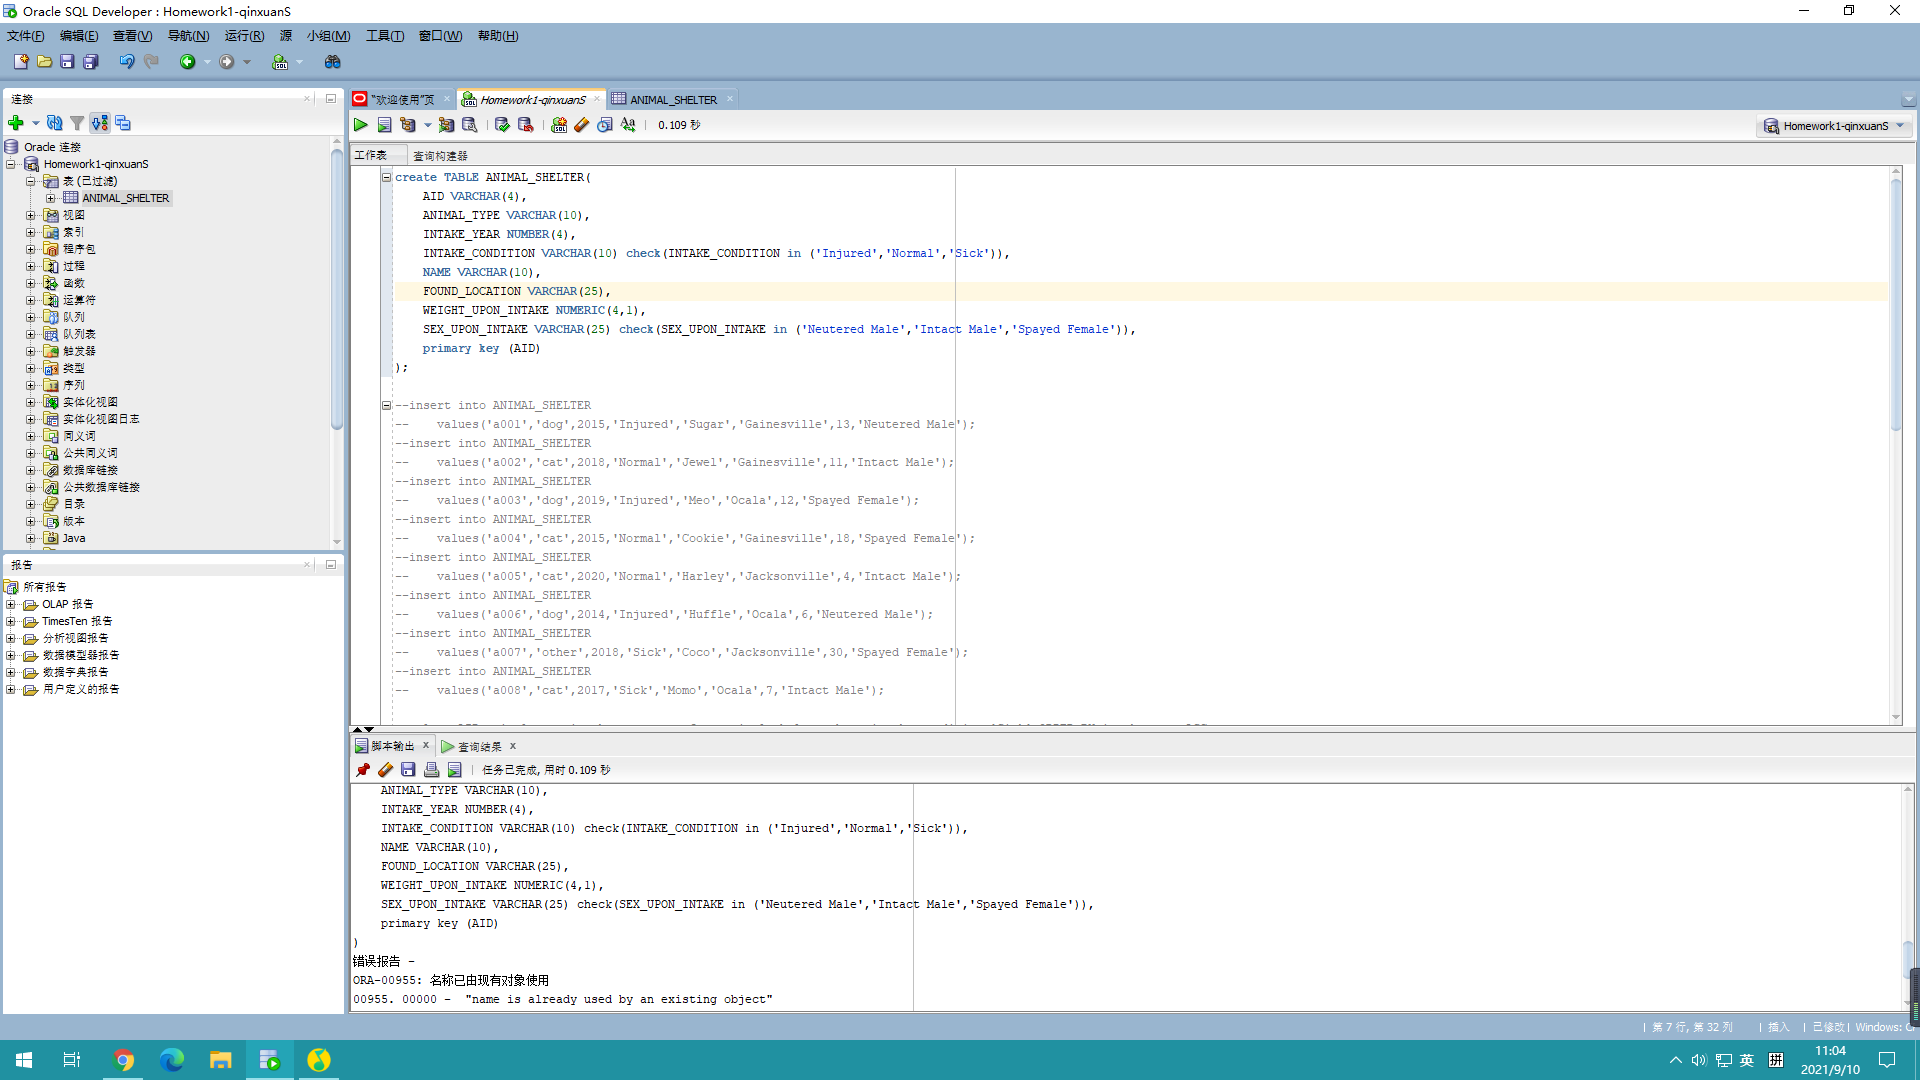
\includegraphics[width=1.0\linewidth]{./document-H1/exercise1/1.1-1}
		\caption{create table}
		\label{1.1-1}
	\end{figure}
	\begin{figure}[H]
		\centering
		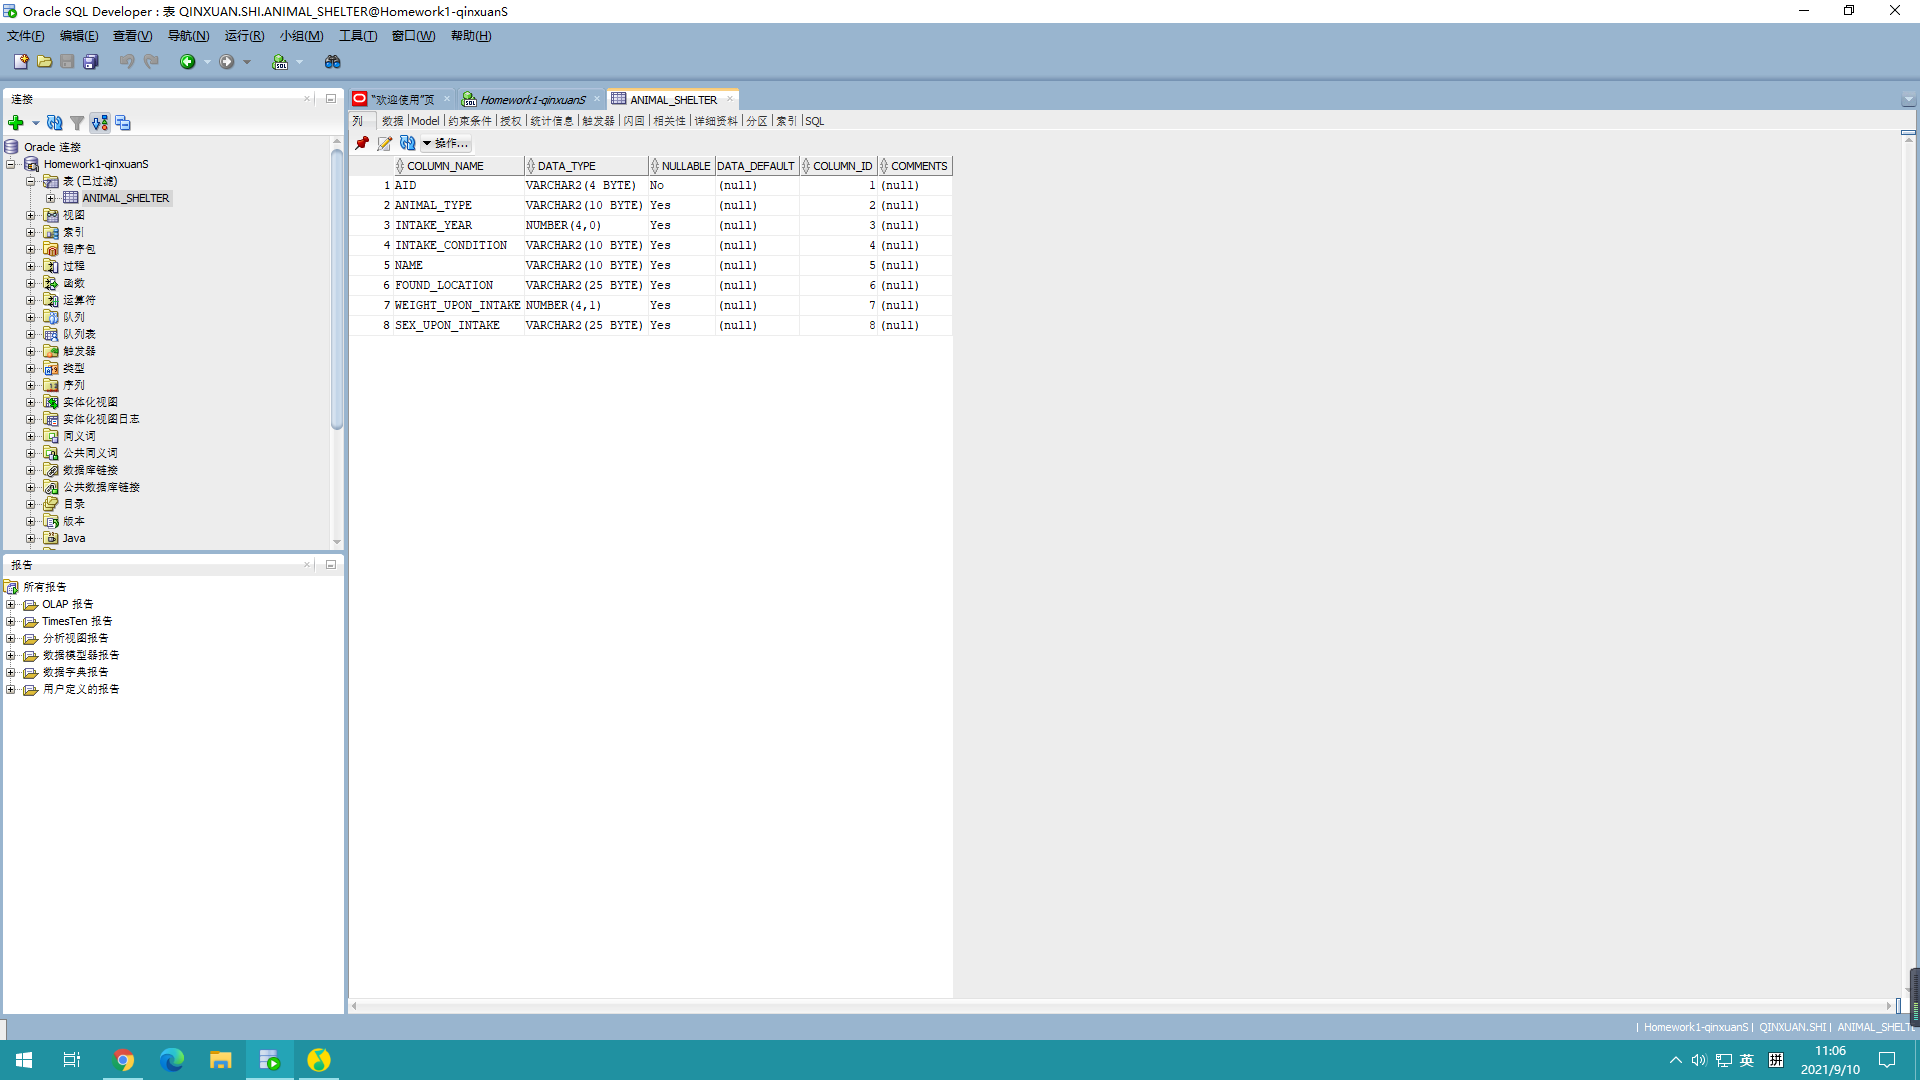
\includegraphics[width=1.0\linewidth]{./document-H1/exercise1/1.1-2}
		\caption{table view}
		\label{1.1-2}
	\end{figure}
	\begin{figure}[H]
		\centering
		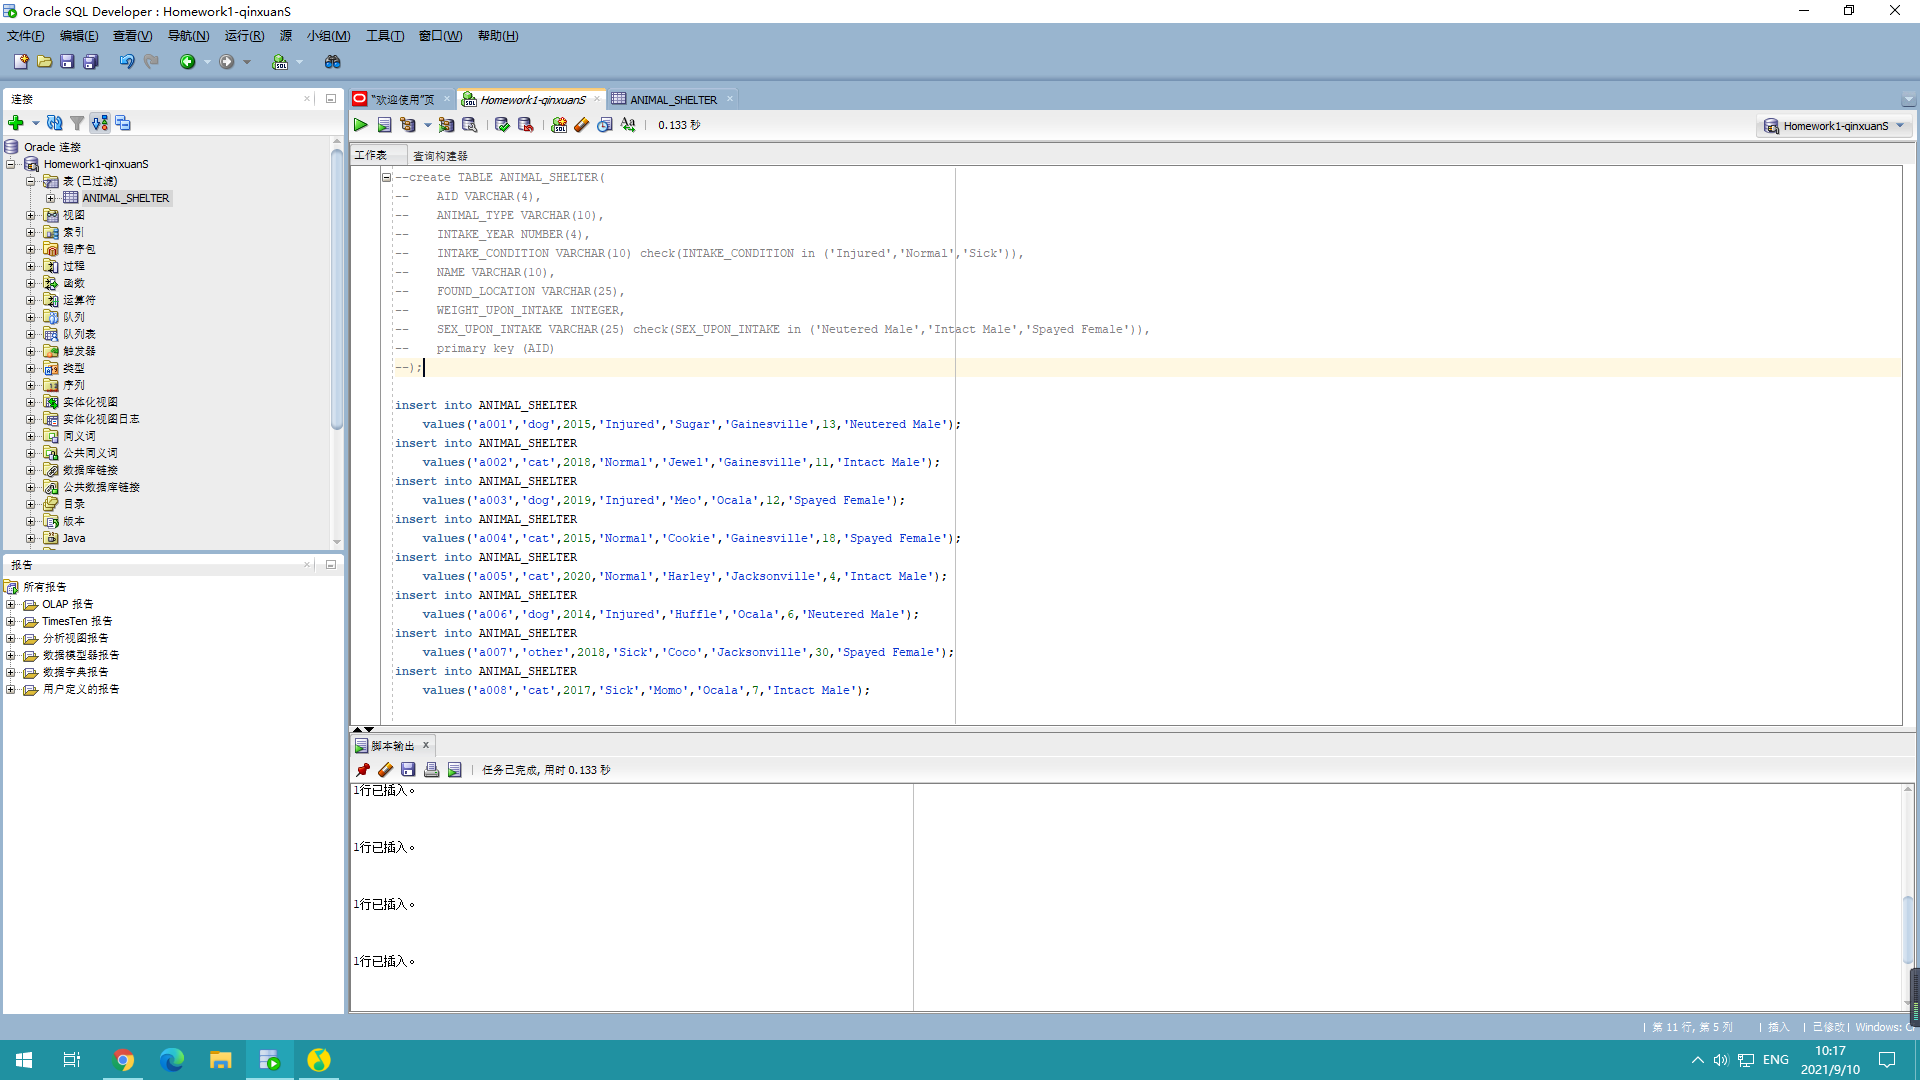
\includegraphics[width=1.0\linewidth]{./document-H1/exercise1/1.1-3}
		\caption{insert data}
		\label{1.1-3}
	\end{figure}
	\begin{figure}[H]
		\centering
		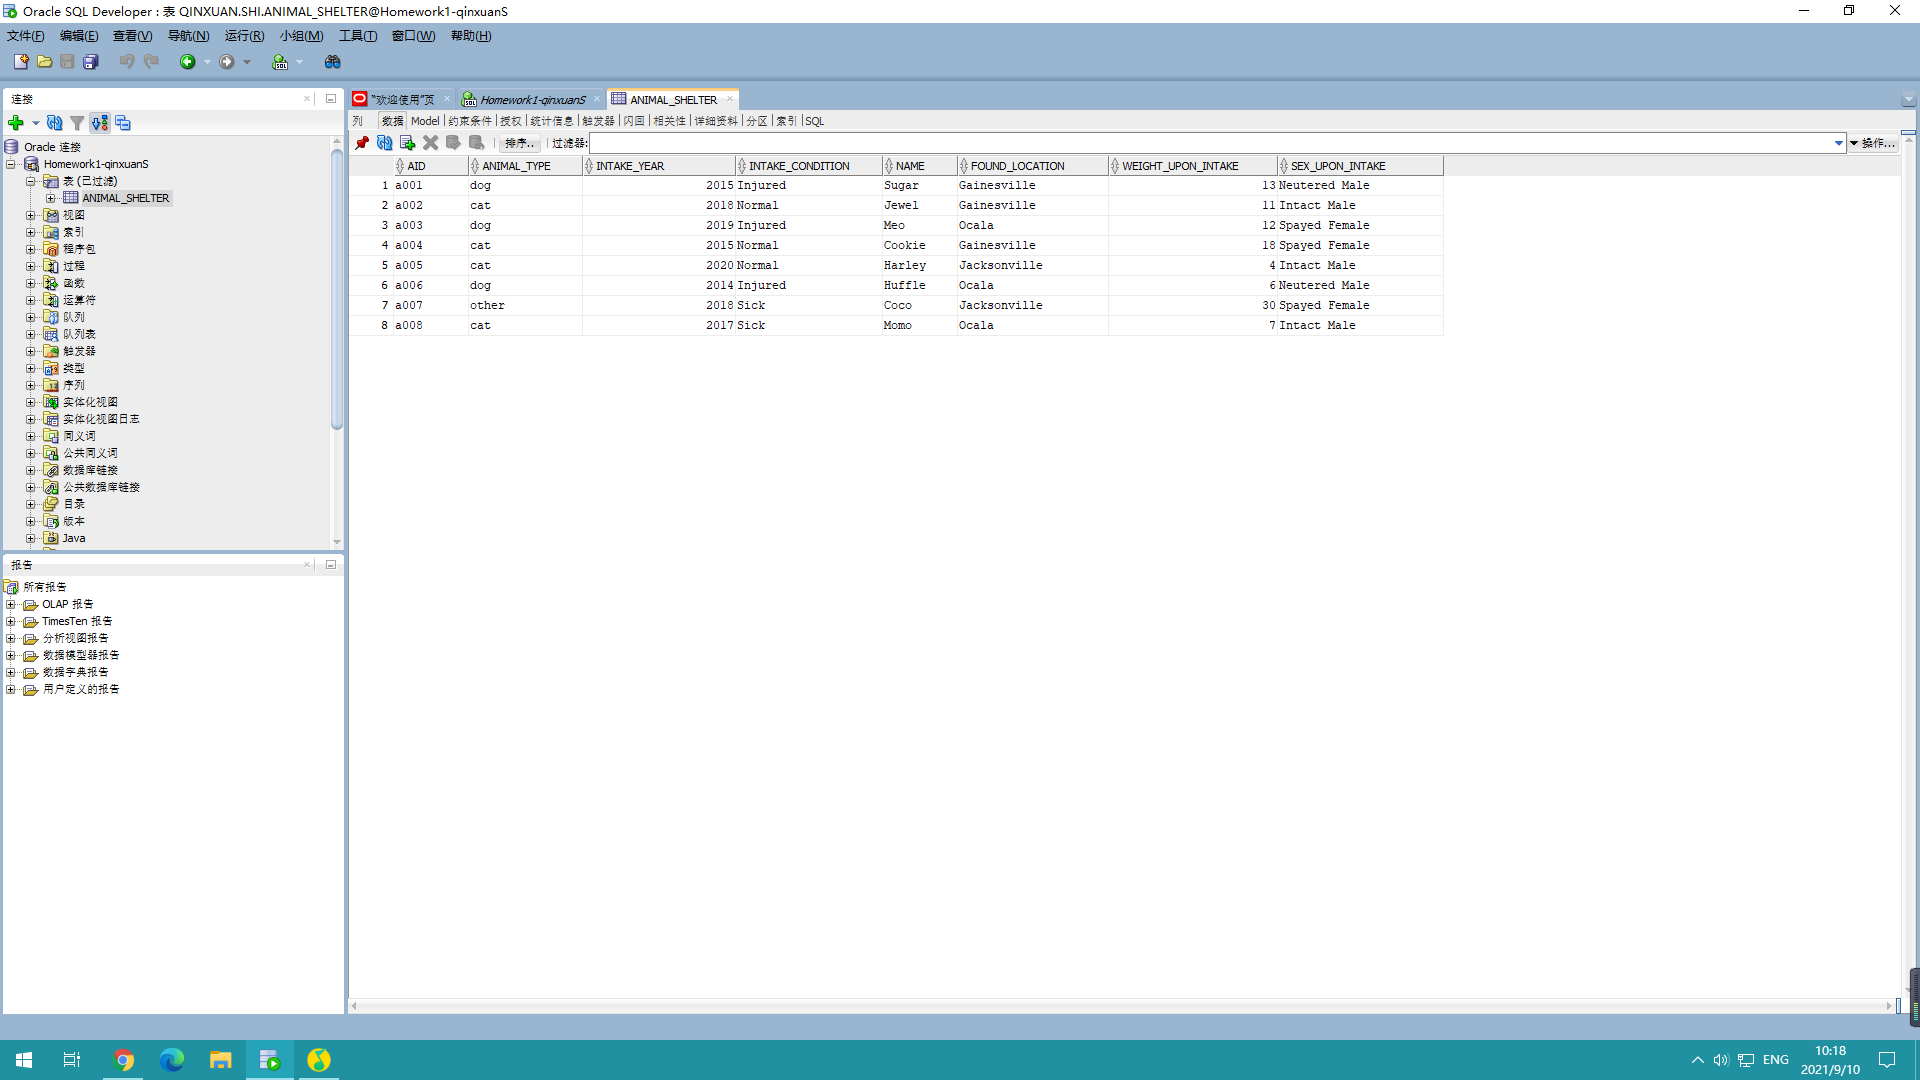
\includegraphics[width=0.95\linewidth]{./document-H1/exercise1/1.1-4}
		\caption{data view}
		\label{1.1-4}
	\end{figure}


(2) SQL queries:
	\begin{lstlisting}[language=] 
  select AID,animal_type,intake_year,name from animal_shelter 
	where intake_condition='Sick' ORDER BY intake_year ASC;
	\end{lstlisting} 
	Output screen snapshots:
	\begin{figure}[H]
		\centering
		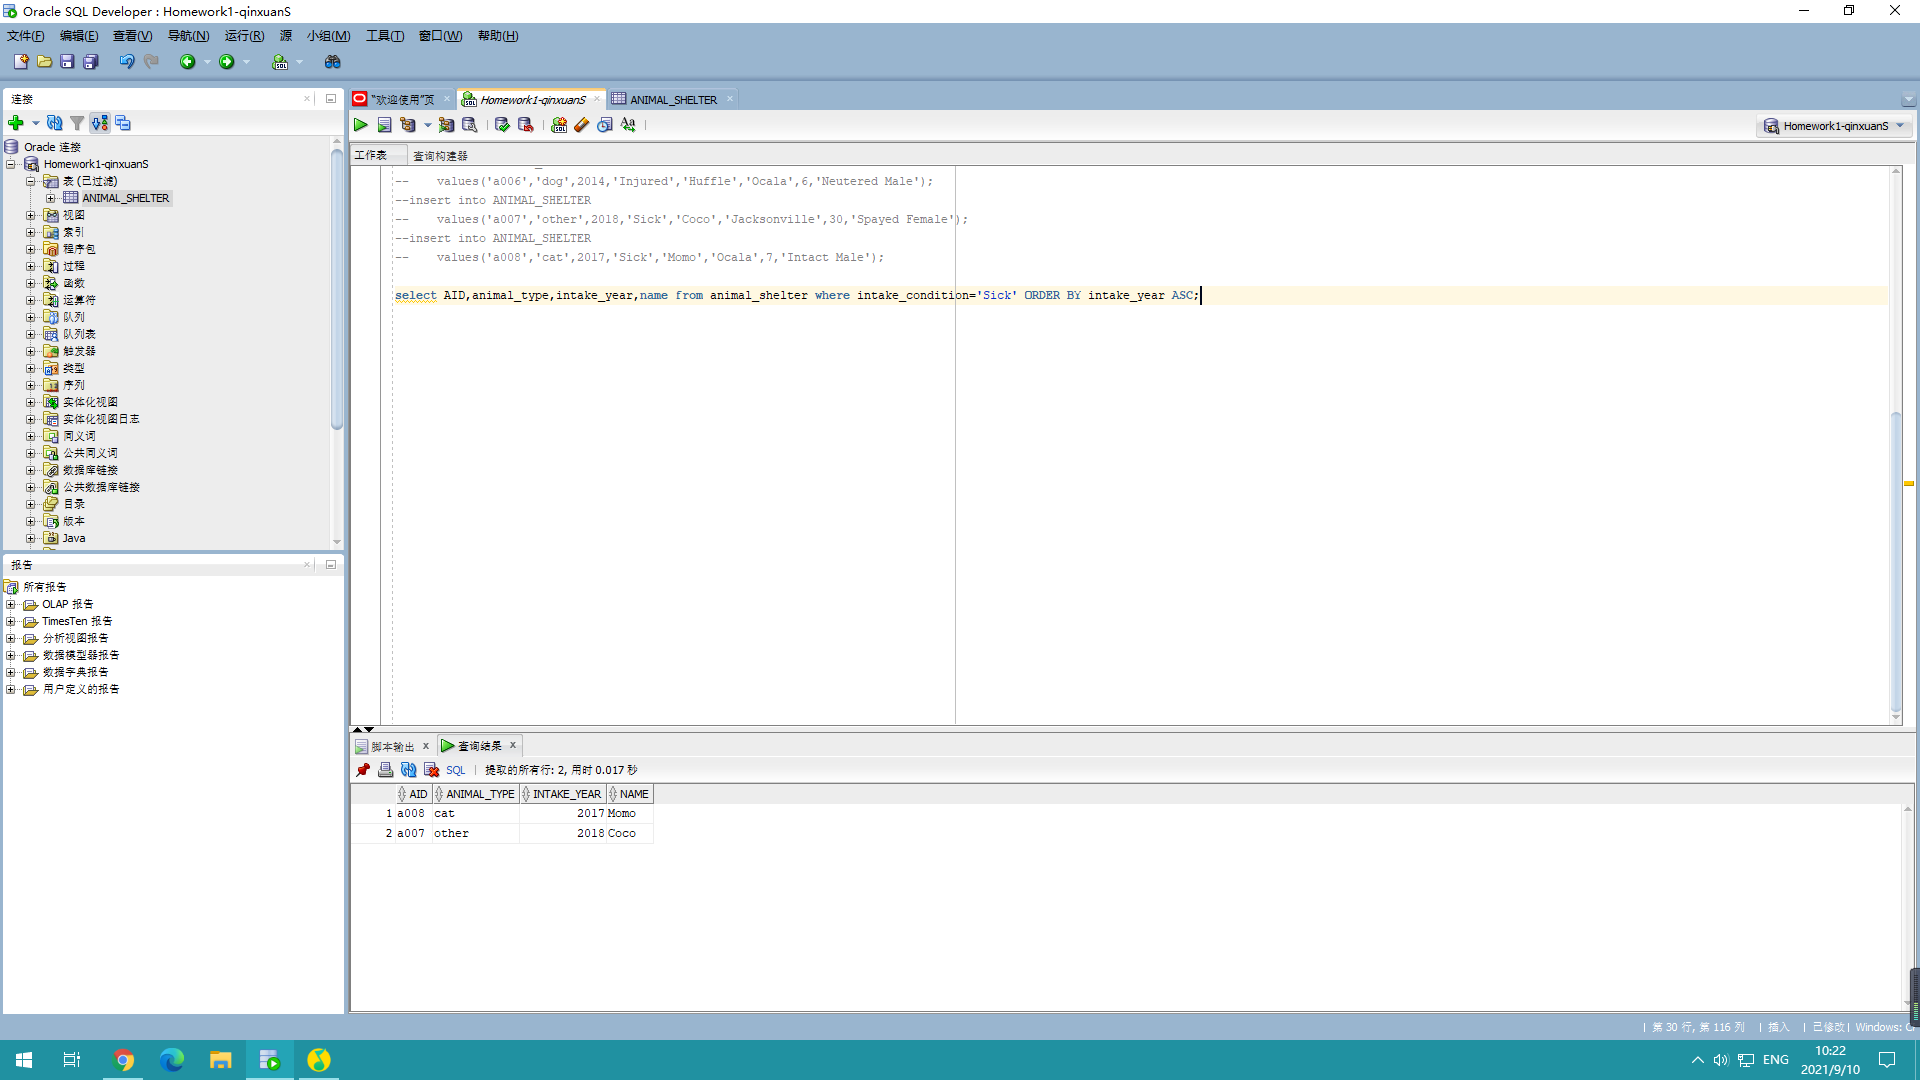
\includegraphics[width=0.95\linewidth]{./document-H1/exercise1/1.2}
		\caption{1.2}
		\label{1.2}
	\end{figure}

(3) SQL queries:
	\begin{lstlisting}[language=] 
  select count(*) from animal_shelter 
    where animal_type='dog' and found_location='Ocala' and intake_year>=2015;
	\end{lstlisting} 
	Output screen snapshots:
	\begin{figure}[H]
		\centering
		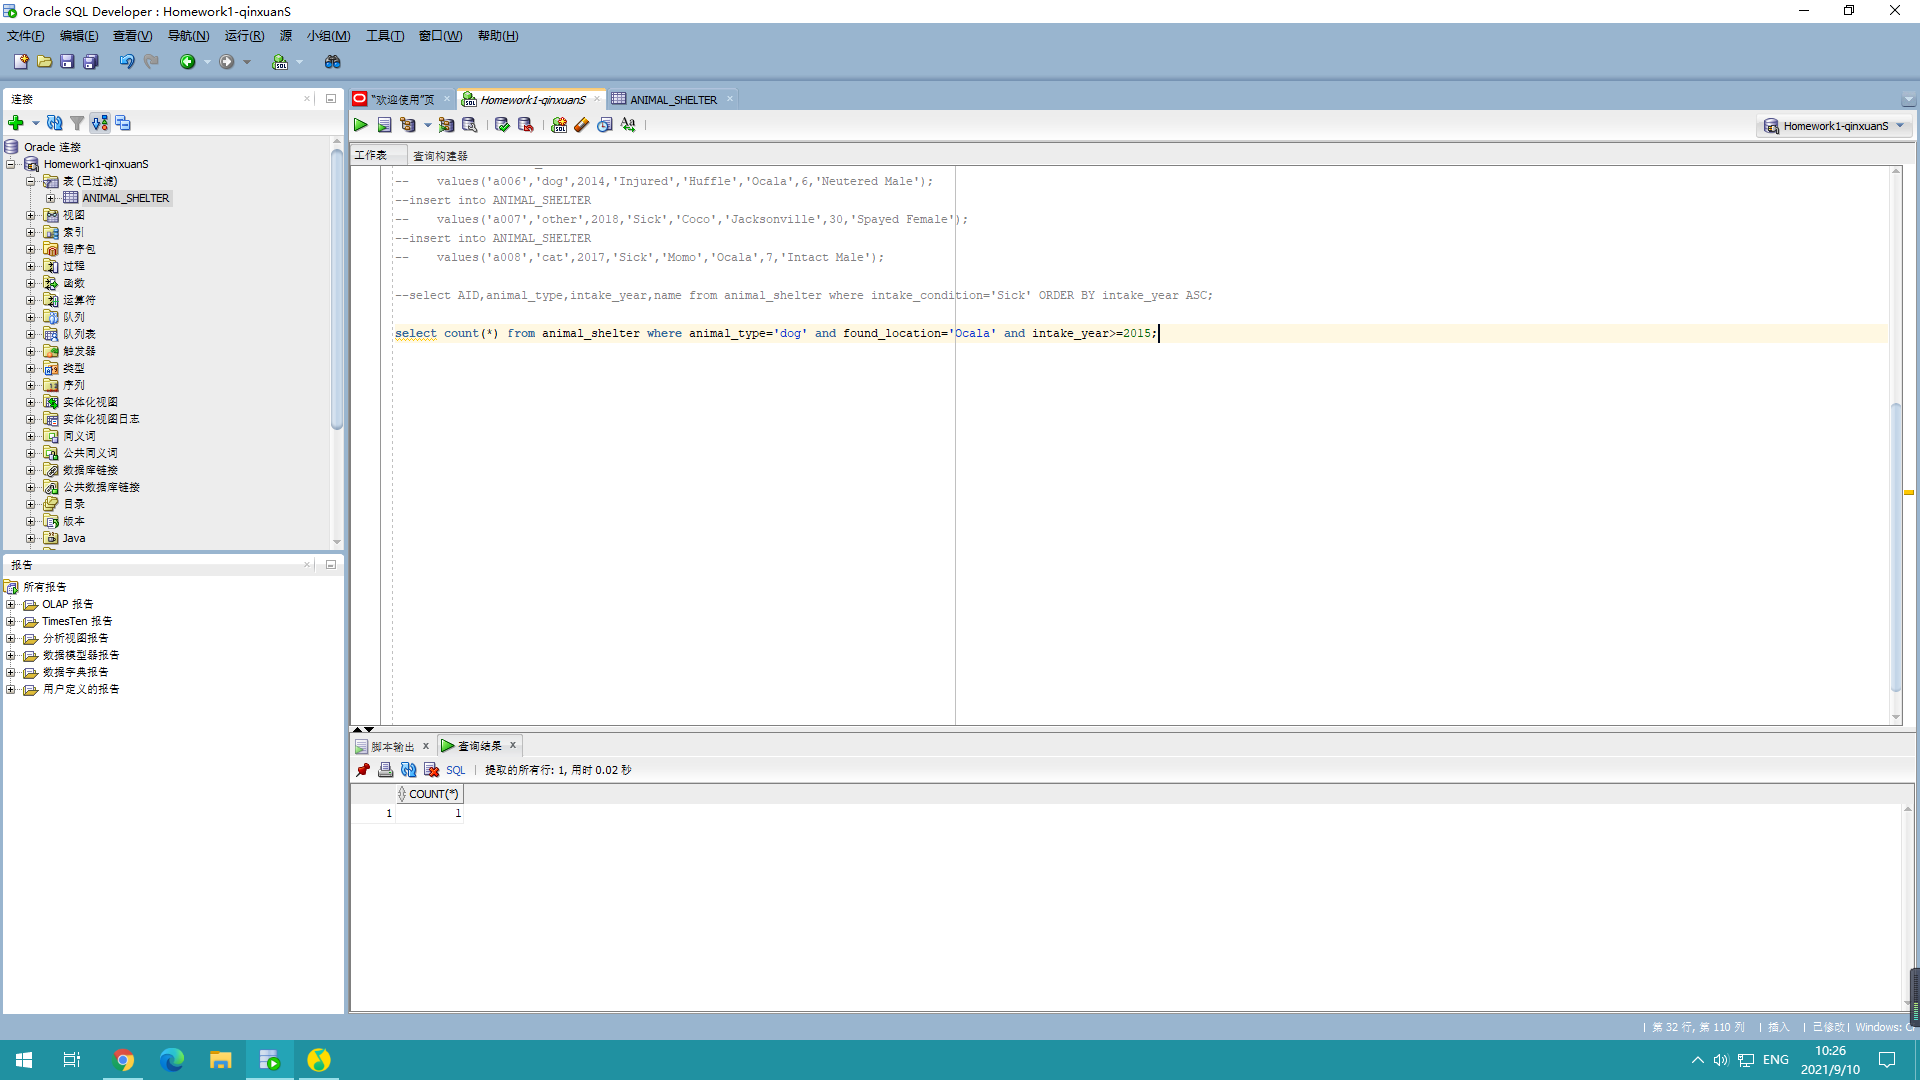
\includegraphics[width=0.90\linewidth]{./document-H1/exercise1/1.3}
		\caption{1.3}
		\label{1.3}
	\end{figure}

(4) SQL queries:
	\begin{lstlisting}[language=] 
  select name,animal_type from animal_shelter 
    where intake_condition='Injured' and found_location='Gainesville' 
    and intake_year>=2014 and intake_year<=2016;	
	\end{lstlisting} 
	Output screen snapshots:
	\begin{figure}[H]
		\centering
		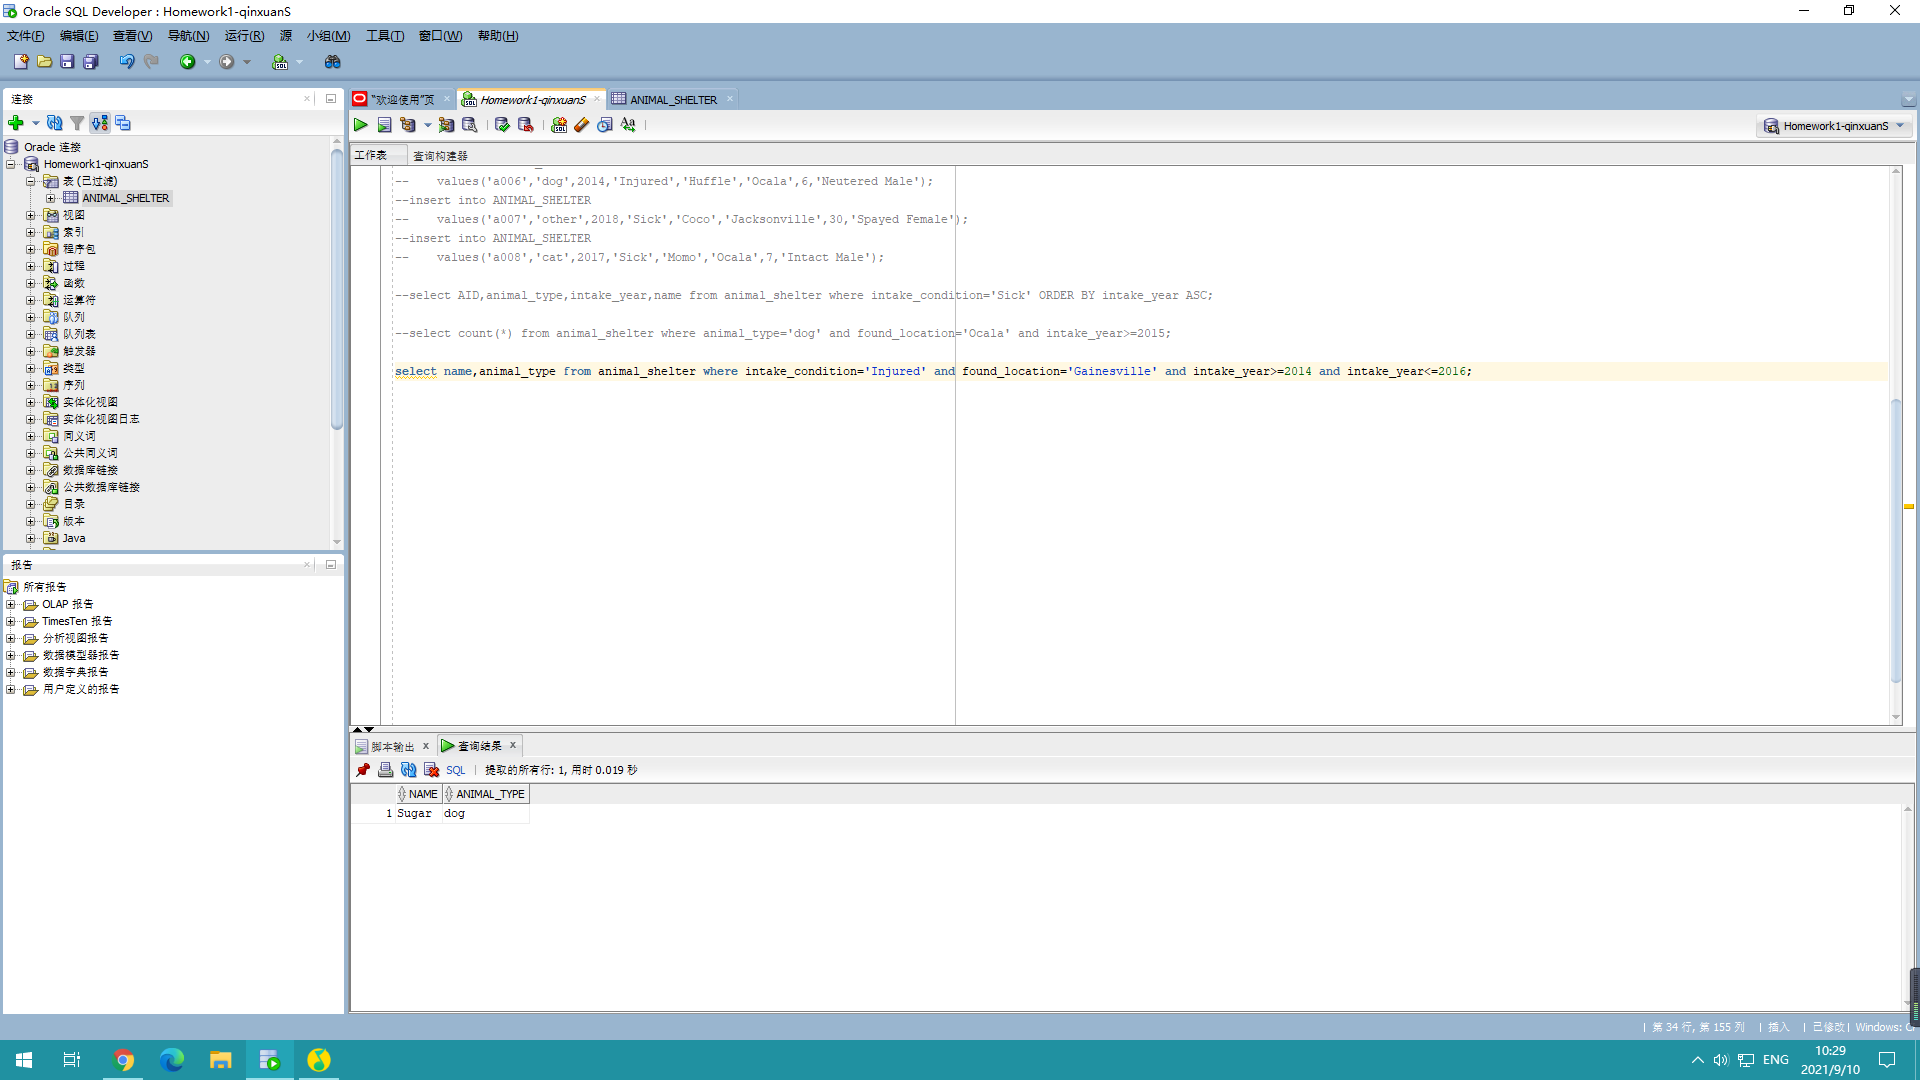
\includegraphics[width=0.95\linewidth]{./document-H1/exercise1/1.4}
		\caption{1.4}
		\label{1.4}
	\end{figure}

(5) SQL queries:
	\begin{lstlisting}[language=] 
  select name,animal_type,intake_condition from animal_shelter
    where AID not in (select AID from animal_shelter where intake_condition='Normal') 
    and (intake_year=2014 or intake_year=2017) and sex_upon_intake='Intact Male';
	\end{lstlisting} 
	Output screen snapshots:
	\begin{figure}[H]
		\centering
		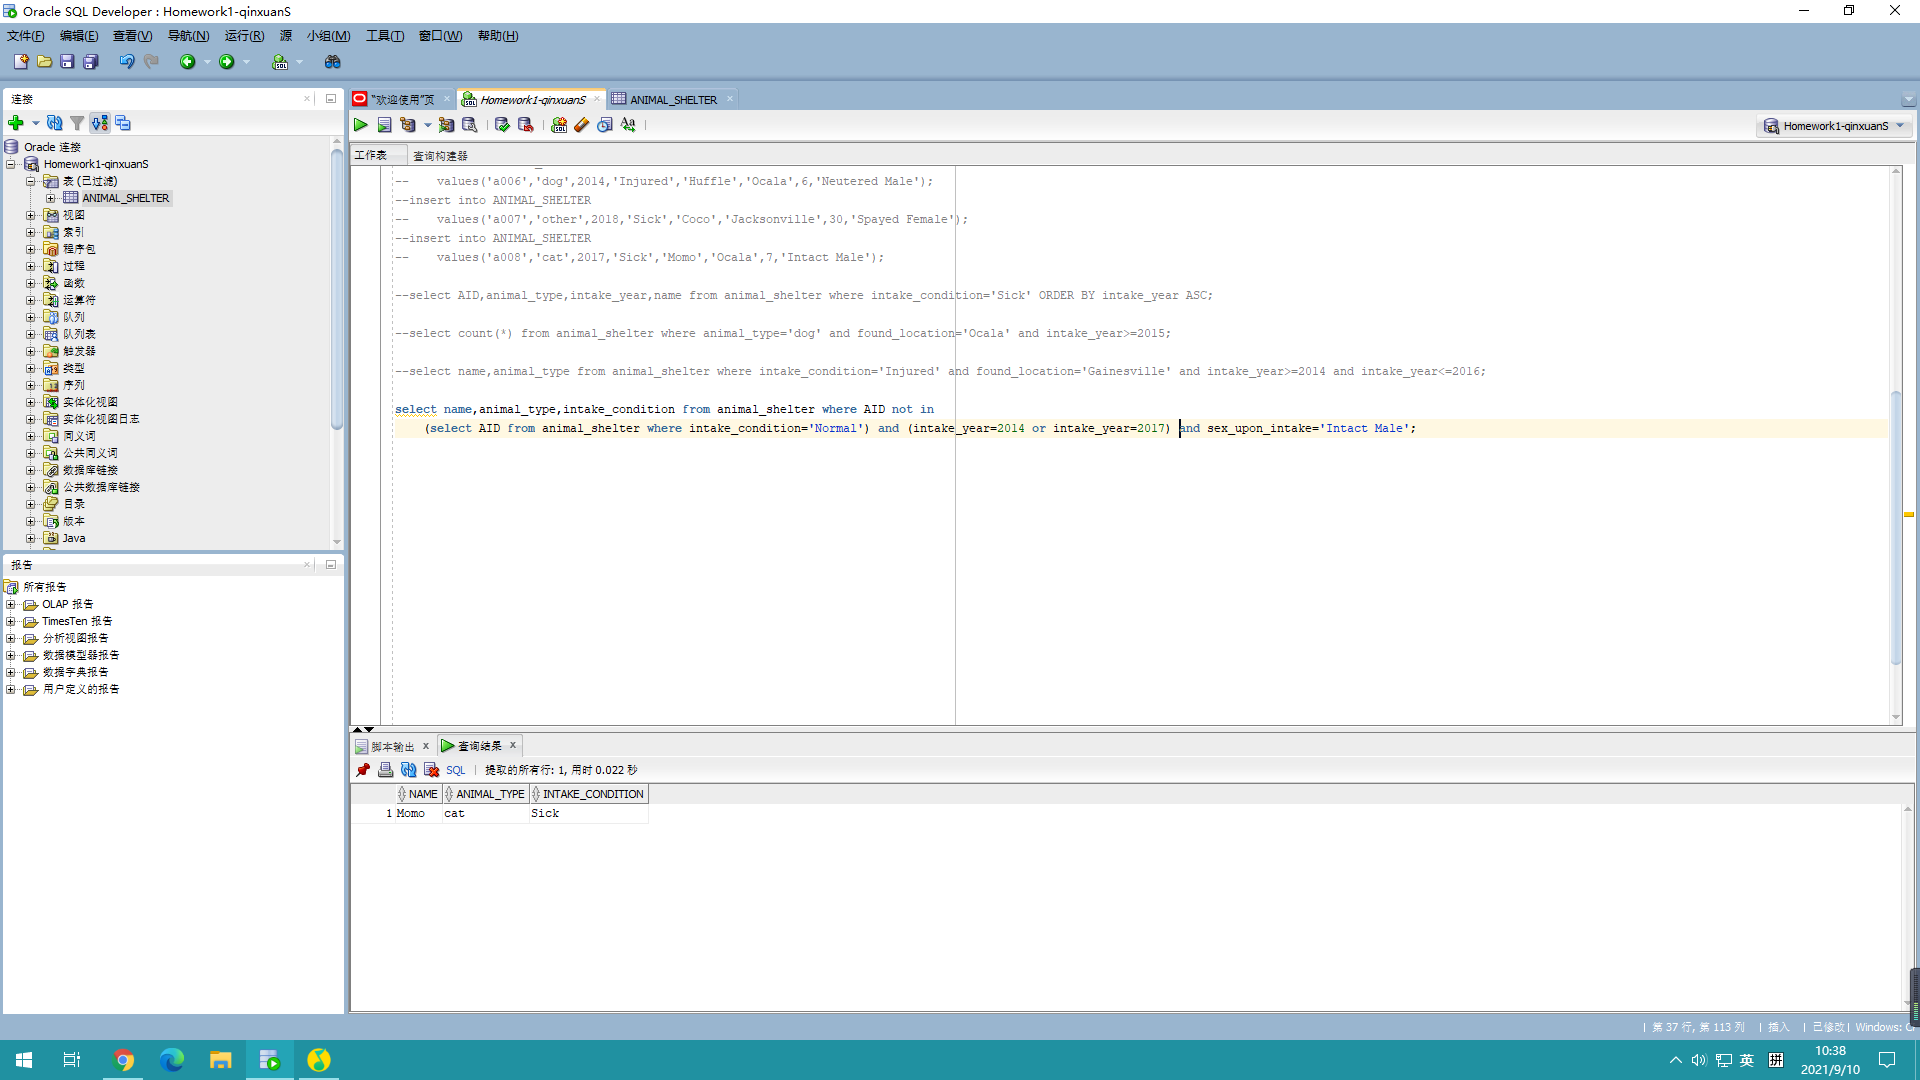
\includegraphics[width=0.88\linewidth]{./document-H1/exercise1/1.5}
		\caption{1.5}
		\label{1.5}
	\end{figure}

(6) SQL queries:
	\begin{lstlisting}[language=] 
  select name,animal_type,intake_year from animal_shelter where 
  (name like '%le%' or name like '%ar%') and (intake_year=2014 or intake_year=2020);
	\end{lstlisting} 
	Output screen snapshots:
	\begin{figure}[H]
		\centering
		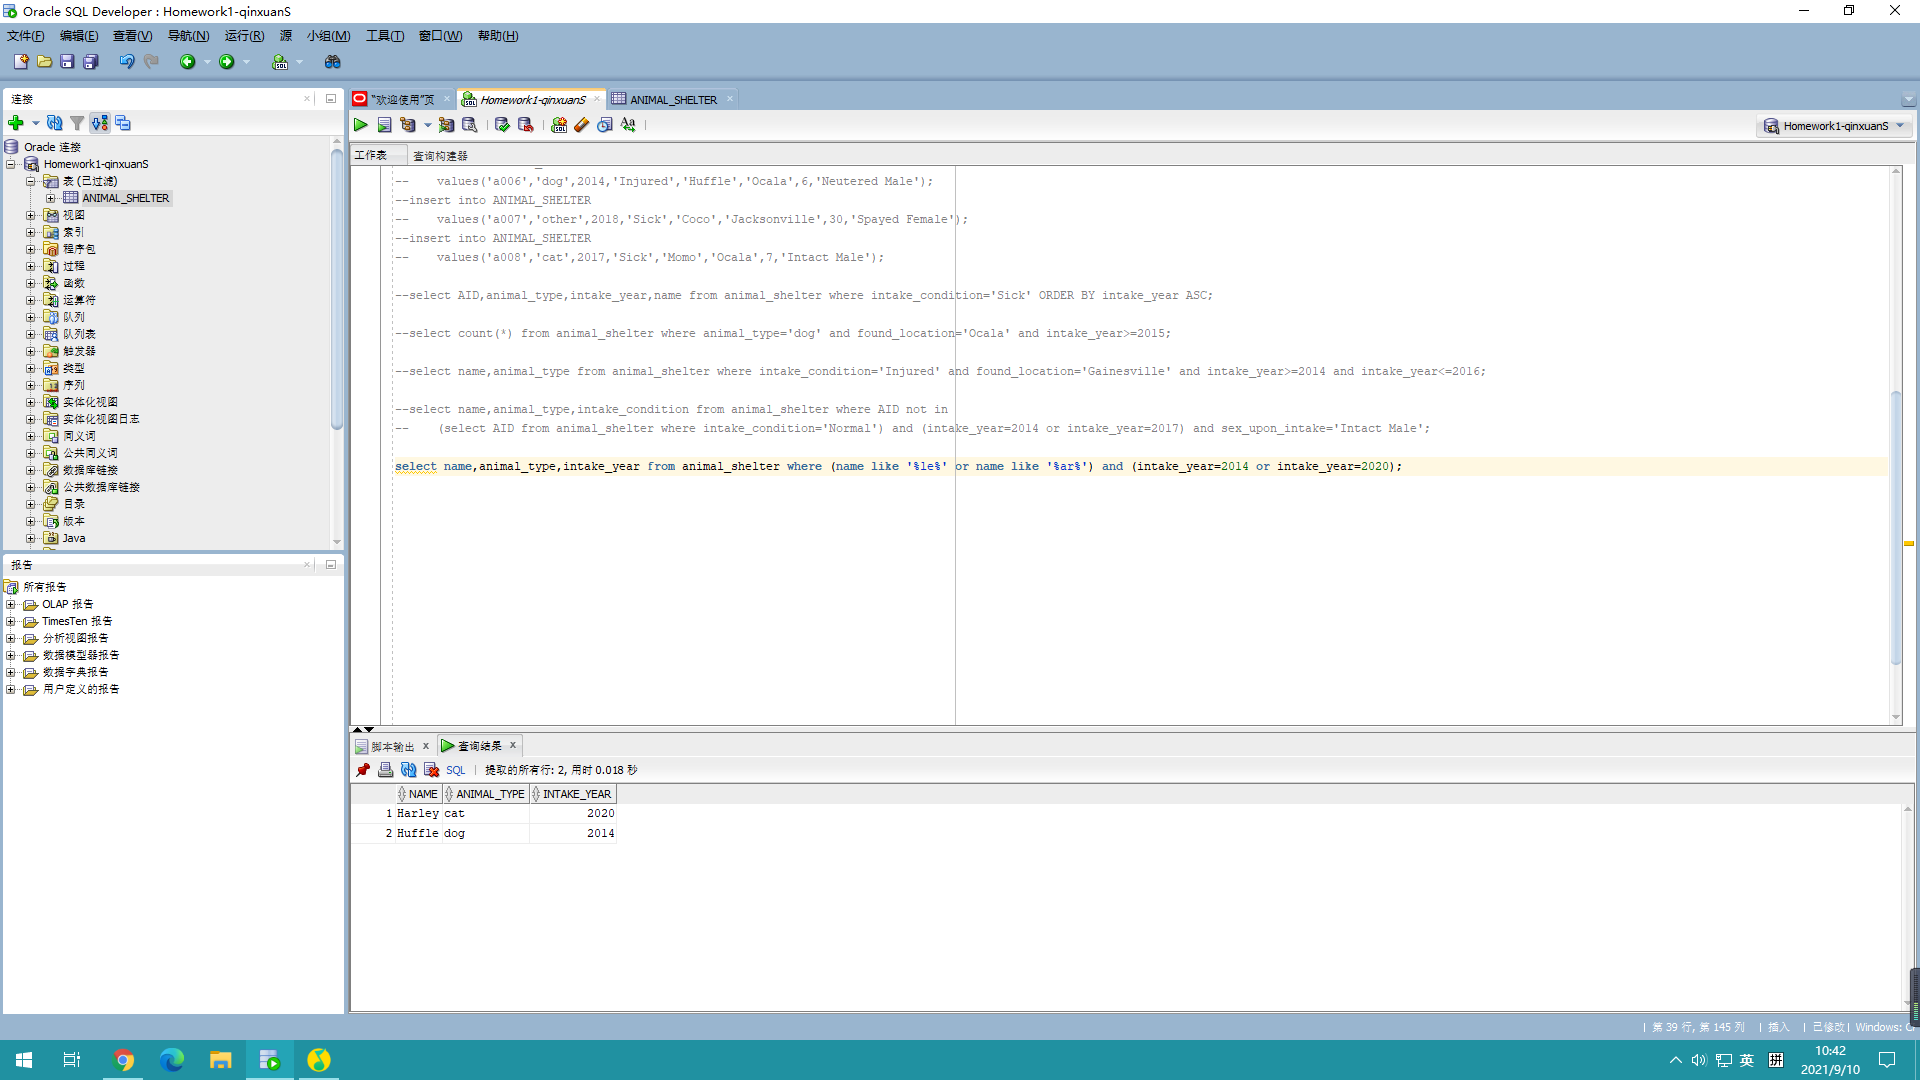
\includegraphics[width=0.88\linewidth]{./document-H1/exercise1/1.6}
		\caption{1.6}
		\label{1.6}
	\end{figure}

(7) SQL queries:
	\begin{lstlisting}[language=] 
  select name,animal_type,intake_year,weight_upon_intake 
  from animal_shelter 
  ORDER BY animal_type ASC, intake_year DESC, weight_upon_intake DESC;
	\end{lstlisting} 
	Output screen snapshots:
	\begin{figure}[H]
		\centering
		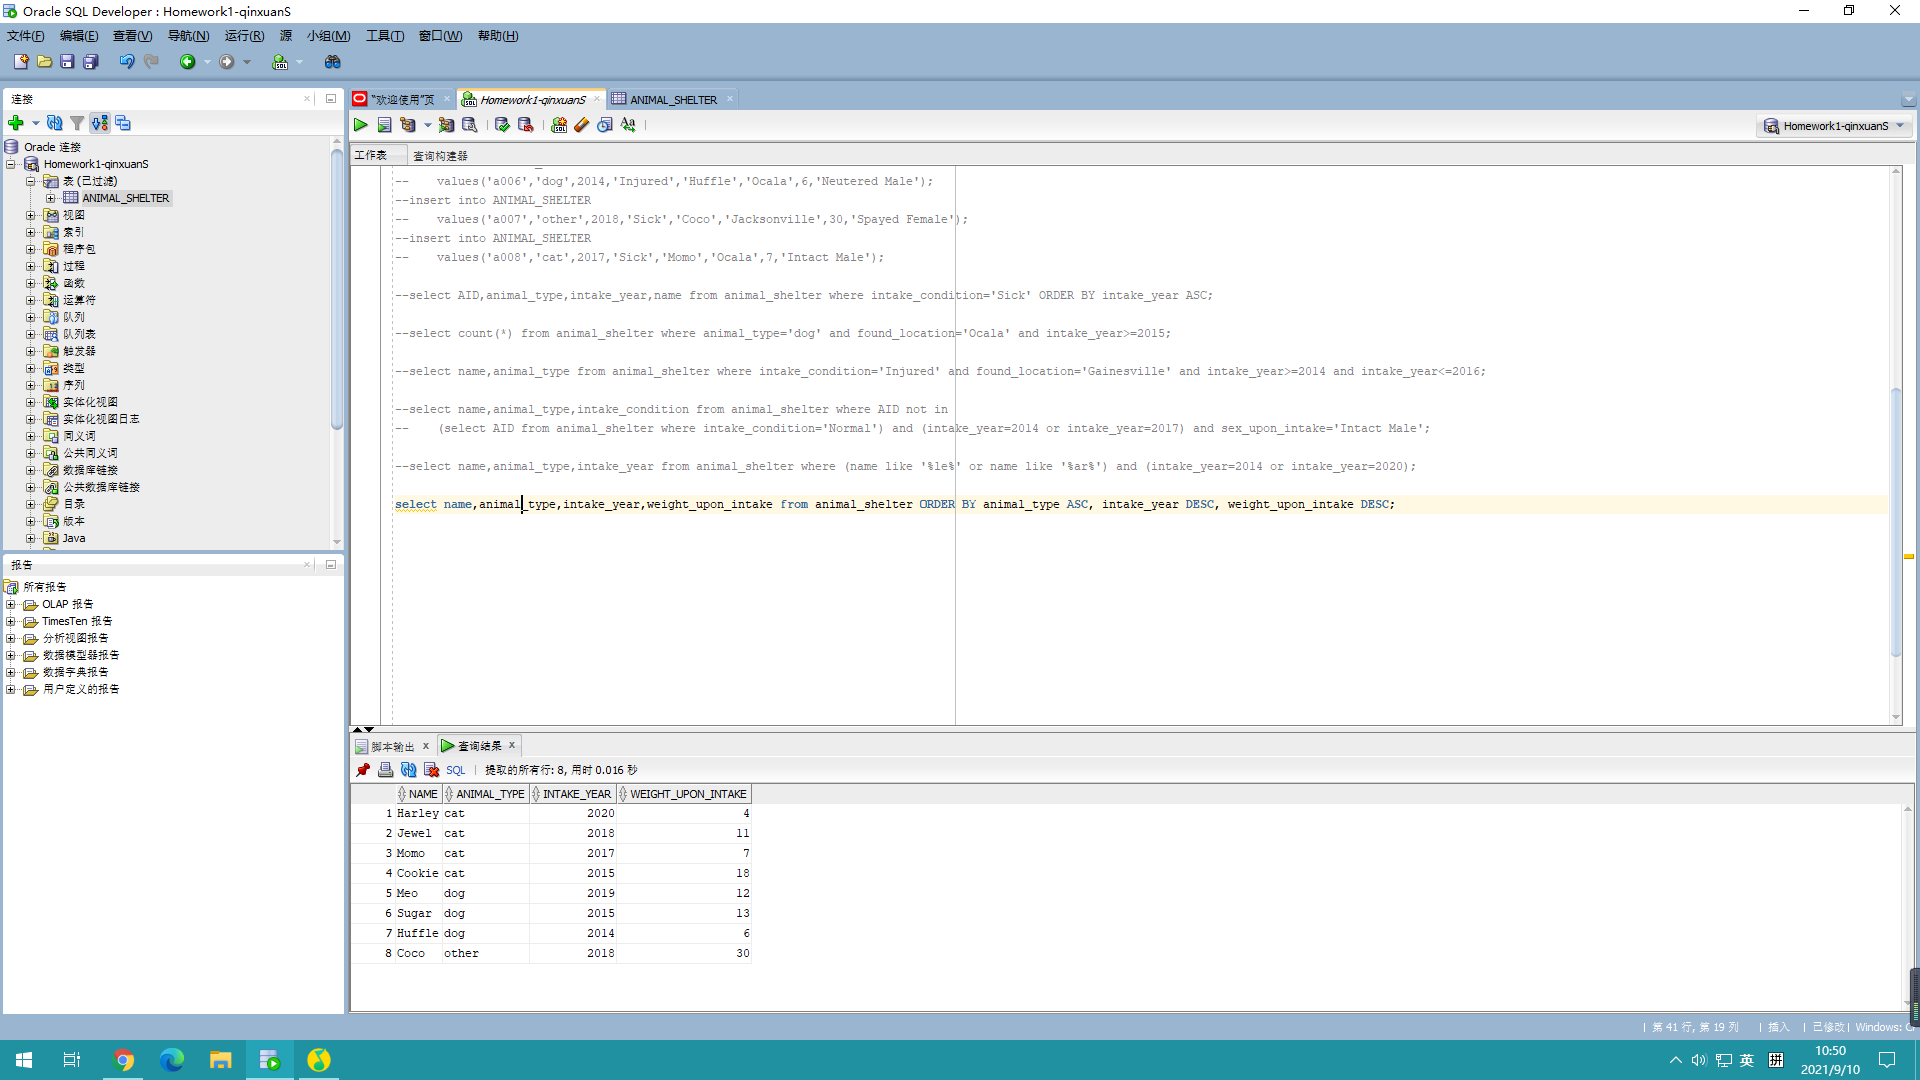
\includegraphics[width=0.9\linewidth]{./document-H1/exercise1/1.7}
		\caption{1.7}
		\label{1.7}
	\end{figure}

(8) SQL queries:
	\begin{lstlisting}[language=] 
  select AVG(weight_upon_intake) as Avg_weight from animal_shelter;
	\end{lstlisting} 
	Output screen snapshots:
	\begin{figure}[H]
		\centering
		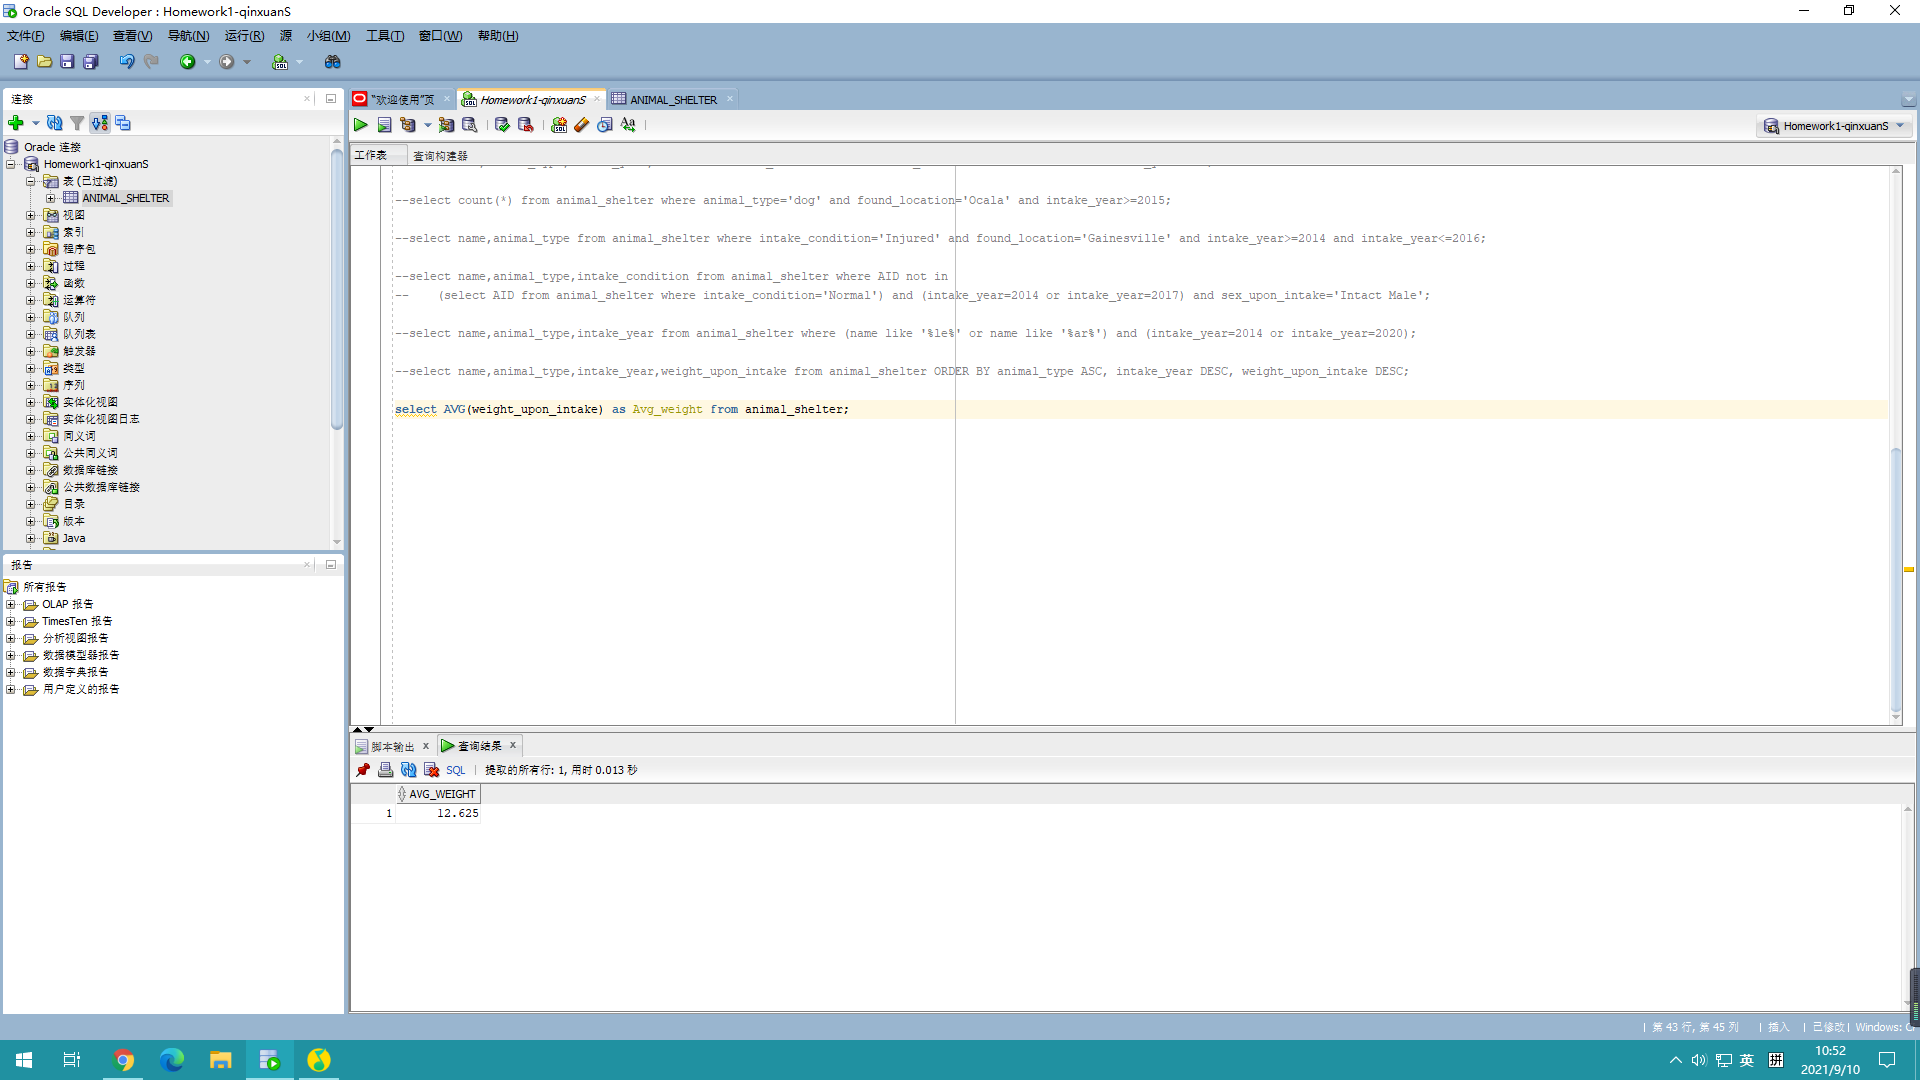
\includegraphics[width=0.9\linewidth]{./document-H1/exercise1/1.8}
		\caption{1.8}
		\label{1.8}
	\end{figure}

(9) SQL queries:
	\begin{lstlisting}[language=] 
  UPDATE animal_shelter SET weight_upon_intake=weight_upon_intake*1.2
    where weight_upon_intake>15;
  select * from animal_shelter;
	\end{lstlisting} 
	Output screen snapshots:
	\begin{figure}[H]
		\centering
		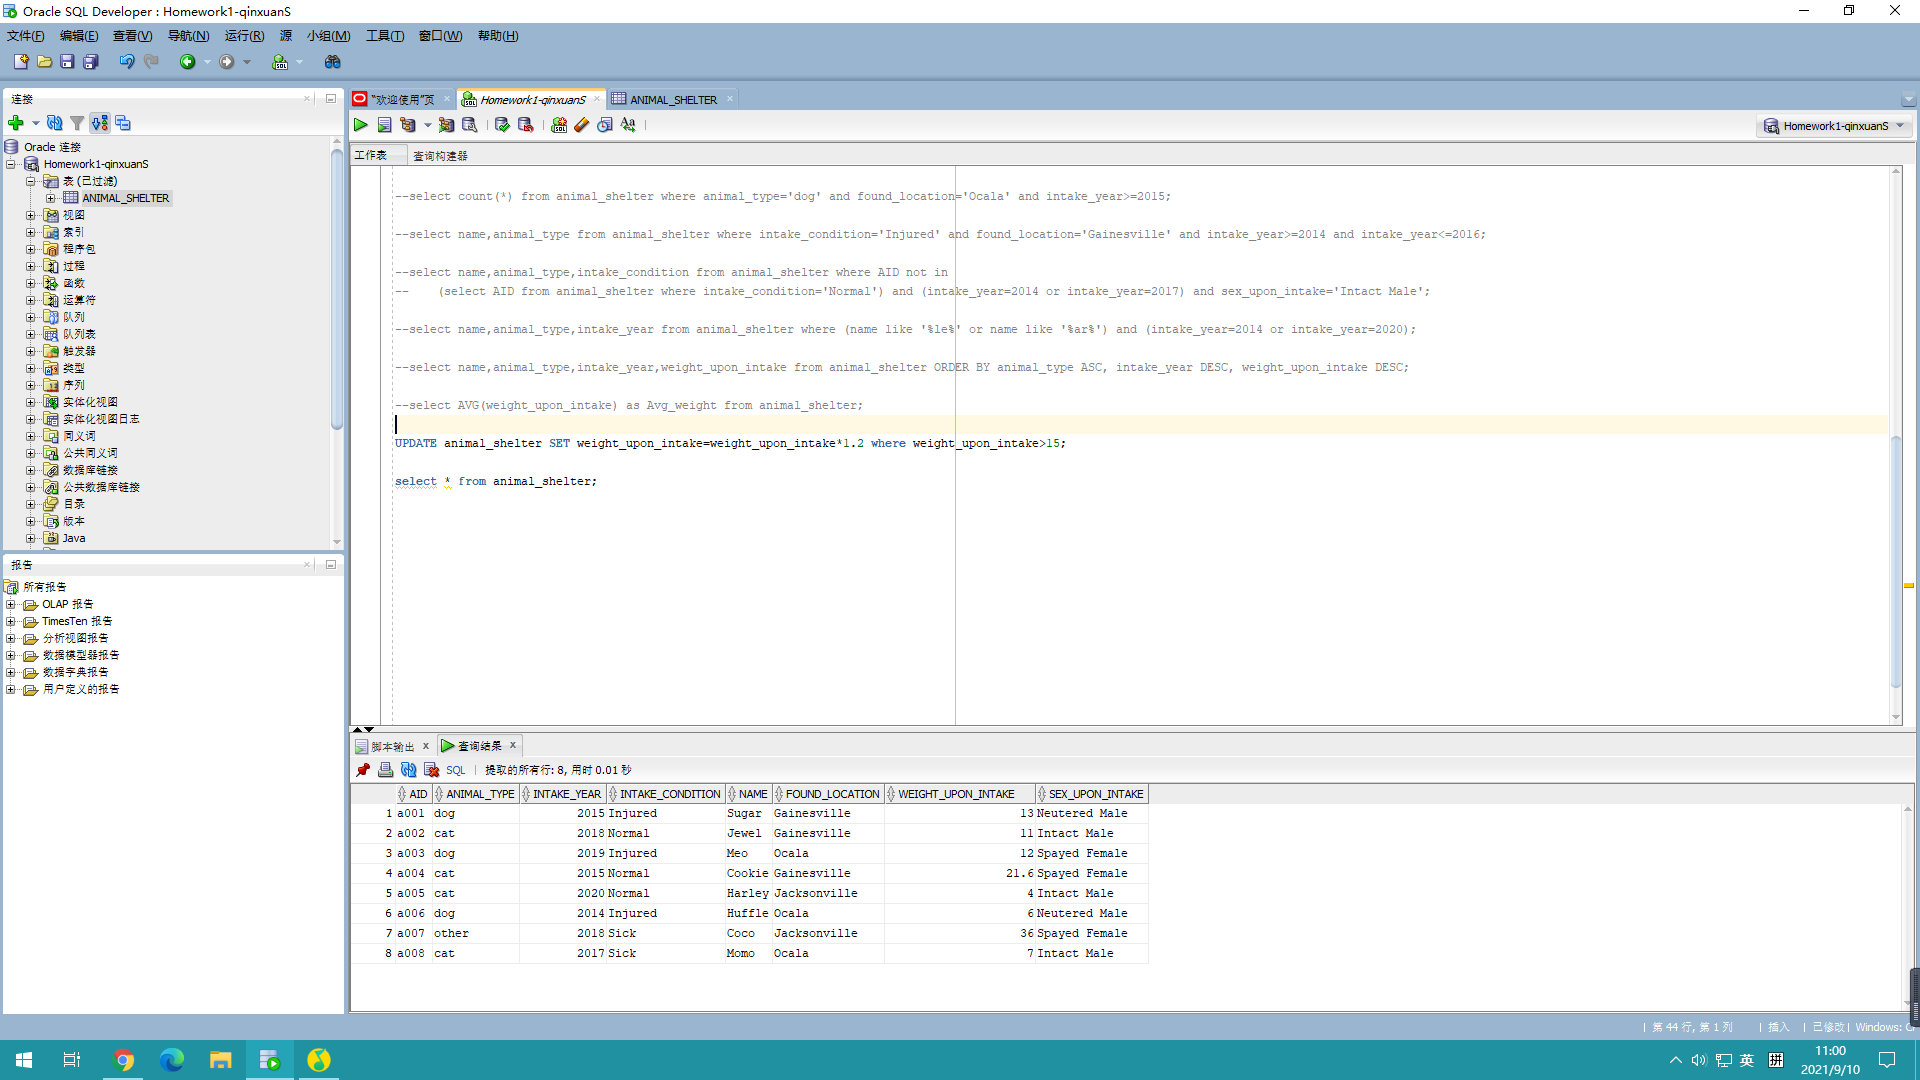
\includegraphics[width=0.90\linewidth]{./document-H1/exercise1/1.9}
		\caption{1.9}
		\label{1.9}
	\end{figure}

\clearpage
\section{Exercise 2}

Entity-Relationship diagram for department management system.
\begin{figure}[H]
	\centering
	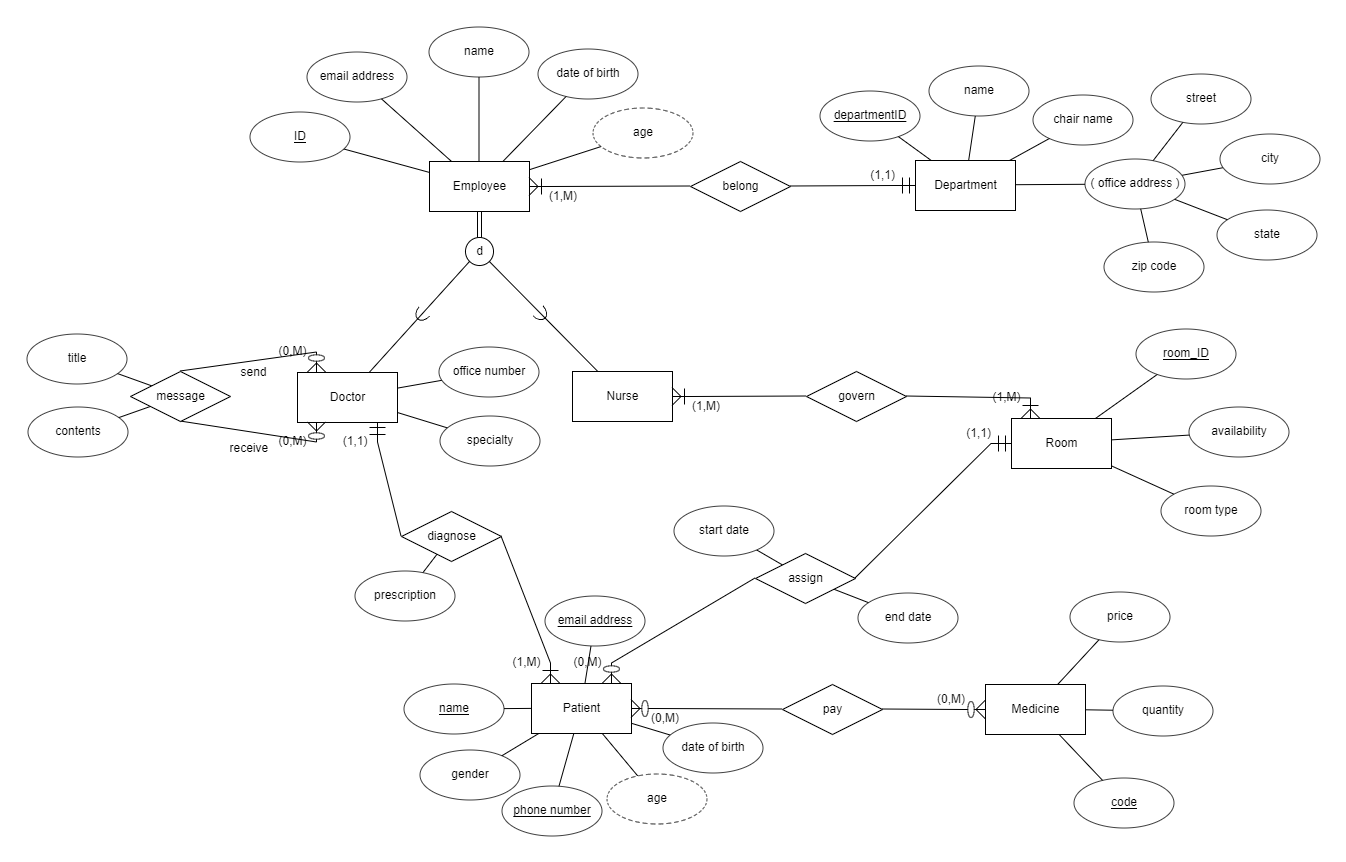
\includegraphics[width=1.13\linewidth]{./document-H1/Homework1-exercise2}
	\caption{Exercise2}
	\label{fig:homework1-exercise2}
\end{figure}

\clearpage
\section{Exercise 3}

Entity-Relationship diagram for online course management system.
\begin{figure}[H]
	\centering
	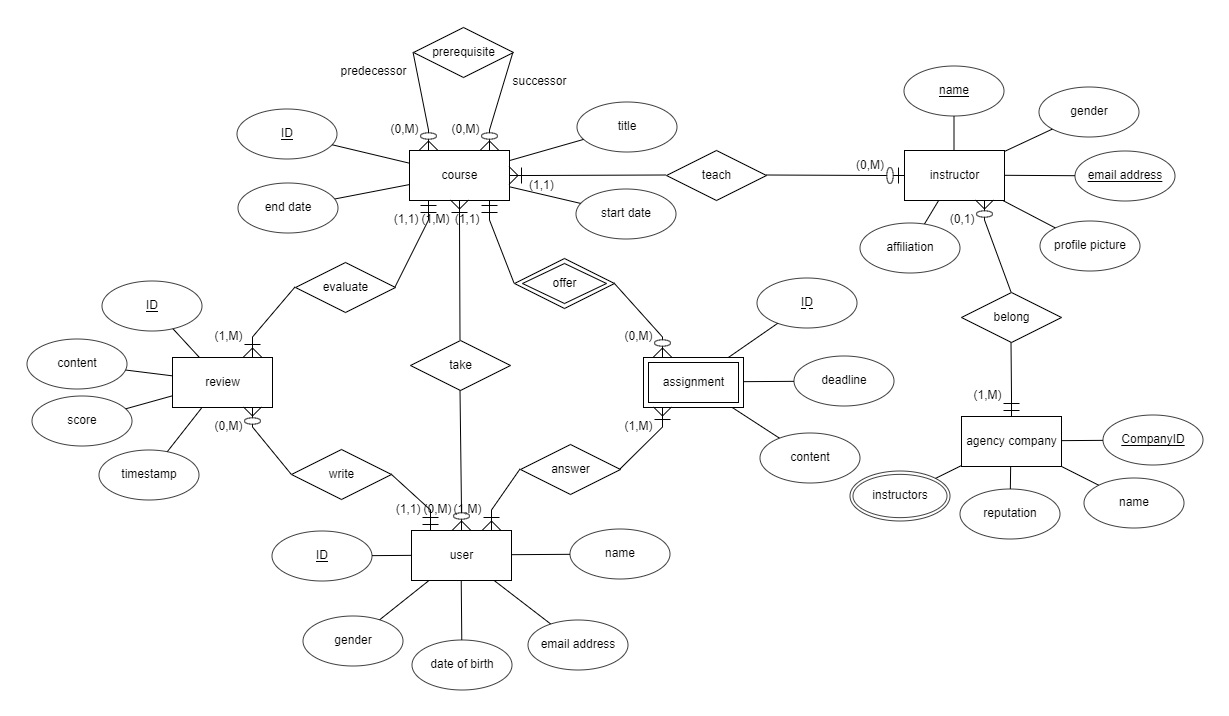
\includegraphics[width=1.13\linewidth]{./document-H1/Homework1-exercise3}
	\caption{Exercise3}
	\label{fig:homework1-exercise3}
\end{figure}

\end{document}
